\documentclass[12pt,a4paper]{book}

\usepackage{amsmath}
\usepackage{amssymb}
\usepackage{tikz}
\usepackage{pgfplots}
\usepackage[siunitx]{circuitikz}
\usepackage{emptypage}
\usepackage{IEEEtrantools}

\usetikzlibrary{scopes}

\pagestyle{plain}

\title
	{
	\huge The IPhO Compendium\\
	\large A Collection of Problems Presented\\ in The International Physics Olympiads
	} 
\date{}

\begin{document}
\maketitle
\frontmatter
\tableofcontents
\mainmatter
\chapter*{I IPhO (Warsaw, 1967)}
\addcontentsline{toc}
{chapter}{I IPhO (Warsaw, 1967)}
\section*{Theoretical problem}
	\subsection*{Problem 1}
	A small ball with mass $M=0.2\text{kg}$ rests on a vertical column with height $h=5\text{m}$. A bullet with mass $m=0.01\text{kg}$, moving with velocity $v_0=500\text{ms}^{-1}$, passes horizontally through the center of the ball. The ball reaches the ground at a distance $s=20\text{m}$. Where does the bullet reach the ground? What part of the kinetic energy of the bullet was converted into heat when the bullet passed through the ball? Neglect resistance of the air, the size of the ball and the bullet. Assume that $g=10\text{m}\text{s}^{-2}$.\\ \\
	\textbf{Solution}\\
	\begin{figure}[!hbtp]
	\centering
	\begin{tikzpicture}
		\draw (0,0) -- (12,0);
		\draw (1.05,0) -- (1.05,1.85) --(0.95,1.85) -- (0.95,0);
		\fill[red] (0.1,2) circle (0.1);
		\draw (0.1,2.4) node {$m,v_0$};
		\draw[->] (0.1,2) -- (0.5,2);
		\fill[blue] (1,2) circle (0.15);
		\draw (1,2.4) node {$M$};
		\draw[<->] (0.75,0) -- (0.75,2);
		\draw (0.5,1) node {$h$};
		\draw[densely dotted] (1,2) parabola (3,0);
		\draw[densely dotted, blue] (2.92,0.15) circle (0.15);
		\draw[<->] (1,-0.25) -- (3,-0.25);
		\draw (2,-0.5) node {$s$};
		\draw[densely dotted] (1,2) parabola (11,0);
		\draw[densely dotted, red] (10.75,0.1) circle (0.1);
		\draw[<->] (1,-0.10) -- (11,-0.10);
		\draw (6,-0.35) node {$d$};
	\end{tikzpicture}
	\caption{Sketch for Problem 1}
	\label{sketch_1_1_1}
	\end{figure}\par
	We will use notation shown in Figure \ref{sketch_1_1_1}.\par
	As no horizontal force acts on the system ball and bullet, the horizontal component of momentum of this system before collision and after collision must be the same,
	\begin{equation*}
		mv_0=mv^{'}+MV
	\end{equation*}
	where $v^{'}$ and $V$ are horizontal component of the velocity of the bullet and of the ball after collision, respectively.\par
	So,
	\begin{equation*}
		v=v_0-\frac{M}{m}V
	\end{equation*}
	From conditions described in the text of the problem it follows that
	\begin{equation*}
		v>V
	\end{equation*}
	After collision, both the ball and the bullet continue a free motion in the gravitational f\mbox{}ield with initial horizontal velocities $v$ and $V$, respectively. Motion of the ball and motion of the bullet are continued for the same time,
	\begin{equation*}
		t=\sqrt{\frac{2h}{g}}
	\end{equation*}
	It is the time of free fall from height $h$.\par
	The distances passed by the ball and bullet during time $t$ are
	\begin{equation*}
		s=Vt\text{ and }d=vt
	\end{equation*}
	respectively. Thus,
	\begin{equation*}
		V=s\sqrt{\frac{g}{2h}}
	\end{equation*}
	Therefore,
	\begin{equation}
		d=v_0\sqrt{\frac{2h}{g}}-\frac{M}{m}s
	\end{equation}
	Numerically,
	\begin{equation*}
		d=100\text{m}
	\end{equation*}
	The total kinetic energy of the system was equal to the initial kinetic energy of the bullet,
	\begin{equation*}
		E_0=\frac{mv_0^{2}}{2}
	\end{equation*}
	Immediately after the collision, the total kinetic energy ot the system is equal to the sum of the kinetic energy of the bullet and the ball,
	\begin{equation*}
		E_m=\frac{mv^{2}}{2}\text{ and }E_M=\frac{MV^{2}}{2}
	\end{equation*}
	Their dif\mbox{}ference, converted into heat, was
	\begin{equation*}
		\Delta E=E_0-(E_m+E_M)
	\end{equation*}
	It is the following part of the initial kinetic energy of the bullet,
	\begin{equation*}
		p=\frac{\Delta E}{E_0}=1-\frac{E_m+E_M}{E_0}
	\end{equation*}
	By using expressions for energies and velocities (quoted earlier) we get
	\begin{equation}
		p=\frac{M}{m}\frac{s^2}{v_0^2}\frac{g}{2h}\Big(2\frac{v_0}{s}\sqrt{\frac{2h}{g}}-\frac{M+m}{m}\Big)
	\end{equation}
	Numerically,
	\begin{equation*}
		p=92.8\text{\%}
	\end{equation*}
	\subsection*{Problem 2}
	Consider an inf\mbox{}inite network consisting of resistors (resistance of each of them is $r$) as shown in Figure \ref{sketch_1_2_1}. Find the resultant resistance $R_{AB}$ between points A and B.\\
	\begin{figure}[!hbtp]
	\centering
	\begin{circuitikz}
		\draw (-0.5,2.5) node {A};
		\draw (0,2.5) to[R, l=$\SI{}{r}$] (2.5,2.5) to[R, l=$\SI{}{r}$] (5,2.5) to[R, l=$\SI{}{r}$] (7.5,2.5) -- (8,2.5);
		\draw[dotted] (8,2.5)-- (9,2.5);
		\draw (2.5,0) to[R, l=$\SI{}{r}$] (2.5,2.5);
		\draw (5,0) to[R, l=$\SI{}{r}$] (5,2.5);
		\draw (7.5,0) to[R, l=$\SI{}{r}$] (7.5,2.5);
		\draw (-0.5,0) node {B};
		\draw (0,0) -- (8,0);
		\draw[dotted] (8,0) -- (9,0);
	\end{circuitikz}
	\caption{Sketch for Problem 2}
	\label{sketch_1_2_1}
	\end{figure}\\ \\
	\textbf{Solution}\\
	It is easy to remark that after removing the left part of the work, shown in Figure \ref{sketch_1_2_2} with the red square, then we receive a network that is identical with the initial network (it is result of the fact that the network is inf\mbox{}inite).
	\begin{figure}[!hbtp]
		\centering
		\begin{circuitikz}
			\draw (-0.5,2.5) node {A};
			\draw (0,2.5) to[R, l=$\SI{}{r}$] (2.5,2.5) to[R, l=$\SI{}{r}$] (5,2.5) to[R, l=$\SI{}{r}$] (7.5,2.5) -- (8,2.5);
			\draw[dotted] (8,2.5)-- (9,2.5);
			\draw (2.5,0) to[R, l=$\SI{}{r}$] (2.5,2.5);
			\draw (5,0) to[R, l=$\SI{}{r}$] (5,2.5);
			\draw (7.5,0) to[R, l=$\SI{}{r}$] (7.5,2.5);
			\draw (-0.5,0) node {B};
			\draw (0,0) -- (8,0);
			\draw[dotted] (8,0) -- (9,0);
			\draw[red] (0.5,-0.75) -- (3,-0.75) -- (3,3.25) -- (0.5,3.25) -- (0.5,-0.75); 
		\end{circuitikz}
		\caption{Auxiliary sketch for Problem 2}
		\label{sketch_1_2_2}
	\end{figure}\par
	Thus, we may use the equivalence shown graphically in Figure \ref{sketch_1_2_3}.
	\begin{figure}[!hbtp]
		\centering
		\begin{circuitikz}
			\draw (-0.5,2.5) node {A};
			\draw (0,2.5) to[R, l=$\SI{}{r}$] (2.5,2.5) -- (5,2.5);
			\draw (2.5,0) to[R, l=$\SI{}{r}$] (2.5,2.5);
			\draw (5,0) to[R, l=$\SI{}{R_{AB}}$] (5,2.5);
			\draw (-0.5,0) node {B};
			\draw (0,0) -- (5,0);
			\draw[red] (0.5,-0.75) -- (3,-0.75) -- (3,3.25) -- (0.5,3.25) -- (0.5,-0.75); 
		\end{circuitikz}
		\caption{Auxiliary sketch for Problem 2}
		\label{sketch_1_2_3}
	\end{figure}\par
	Algebraically, this equivalence can be written as
	\begin{equation*}
		R_{AB}=r+\frac{1}{\frac{1}{r}+\frac{1}{R_{AB}}}
	\end{equation*}
	Thus
	\begin{equation*}
		R_{AB}^2-rR_{AB}-r^2=0
	\end{equation*}
	This equation has two solutions,
	\begin{equation*}
		R_{AB}=\frac{1}{2}(1\pm\sqrt{5})r
	\end{equation*}
	The solution corresponding to "-" in the above formula is negative, while resistance must be positive. So, we reject it. Finally, we receive
	\begin{equation}
		R_{AB}=\frac{1}{2}(1+\sqrt{5})r
	\end{equation}
	\subsection*{Problem 3}
	Consider two identical homogeneous balls, A and B, with the same initial temperatures. One of them is at rest on a horizontal plane, while the second one hangs on a thread (Figure \ref{sketch_1_3_1}). The same quantities of heat have been supplied to both balls. Are the f\mbox{}inal temperatures of the balls the same or not? Justify your answer. (All kinds of heat losses are negligible.)
	\begin{figure}[!hbtp]
		\centering
		\begin{tikzpicture}
			\draw[thick] (0,4) -- (3,4);
			\draw (1.5,4) -- (1.5,3);
			\draw (1.5,2) circle (1);
			\draw (1.5,2) node {A};
			\draw[thick] (5,0) -- (8,0);
			\draw (6.5,1) circle (1);
			\draw (6.5,1) node {B};
		\end{tikzpicture}
		\caption{Sketch for Problem 3}
		\label{sketch_1_3_1}
	\end{figure}\\ \\
	\textbf{Solution}\\
	As regards the text of the problem, the sentence \emph{"The same quantities of heat have been supplied to both balls."} is not too clear. We will follow intuitive understanding of this sentence, i.e. we will assume that both systems (A - the hanging ball and B - the ball resting on the plane) received the same portion of energy from outside. One should realize, however, that it is not the only possible interpretation.\par
	When the balls are warmed up, their mass centers are moving as the radii of the balls are changing. The mass center of the ball A goes down, while the mass center of the ball B goes up. It is shown in Figure \ref{sketch_1_3_2}(scale is not conserved).\par
	\begin{figure}[!hbtp]
		\centering
		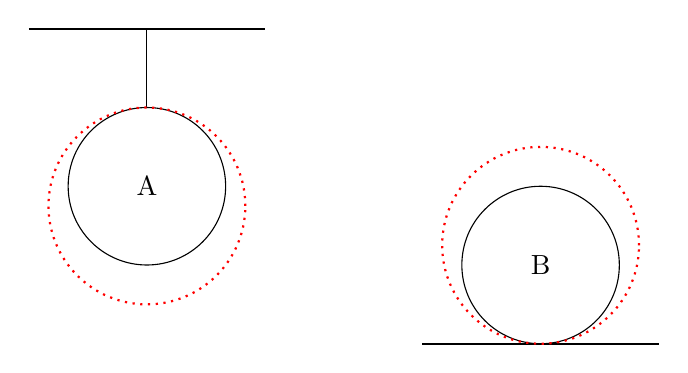
\begin{tikzpicture}
			\draw[thick] (0,4) -- (3,4);
			\draw (1.5,4) -- (1.5,3);
			\draw (1.5,2) circle (1);
			\draw[thick,dotted,red] (1.5,1.75) circle (1.25);
			\draw (1.5,2) node {A};
			\draw[thick] (5,0) -- (8,0);
			\draw (6.5,1) circle (1);
			\draw[thick,dotted,red] (6.5,1.25) circle (1.25);
			\draw (6.5,1) node {B};
		\end{tikzpicture}
		\caption{Auxiliary sketch for Problem 3}
		\label{sketch_1_3_2}
	\end{figure}
	Displacement of the mass center corresponds to a change of the potential energy of the ball in the gravitational f\mbox{}ield.\par
	In case of the ball A the potential energy decreases. From the 1$^\text{st}$ principle of thermodynamics, it corresponds to additional heating of the ball.\par
	In case of the ball B the potential energy increases. From the 1$^\text{st}$ principle of thermodynamics it corresponds to some "losses of the heat provided" for performing a mechanical work necessary to rise the ball. The net result is that the f\mbox{}inal temperature of the ball B should be lower than the f\mbox{}inal temperature of the ball A.\par
	The above ef\mbox{}fect is very small. For example, one my f\mbox{}ind (see later) that for balls made of lead, with radius 10cm, and portion of heat equal to 50kcal, the dif\mbox{}ference of the f\mbox{}inal temperature of the balls is of order $10^{-5}$K. For spatial and time f\mbox{}luctuations, such small quantity practically cannot be measured.\par
	Calculation of the dif\mbox{}ference of the f\mbox{}inal temperatures was not required from the participants. Nevertheless, we present it here as an element of discussion.\par
	We may assume that the work against the atmospheric pressure can be neglected. It is obvious that this work is small. Moreover, it is almost the same for both balls. So, it should not af\mbox{}fect the dif\mbox{}ference of the temperatures substantially. We will assume that such quantities as specif\mbox{}ic heat of the lead and coef\mbox{}f\mbox{}icient of thermal expansion of lead are constant (i.e. do not depend on temperature).\par
	The heat used for changing the temperatures of balls may be written as
	\begin{equation*}
		Q_i=mc\Delta t_i\text{, where }i=A\text{ or } B
	\end{equation*}
	Here, $m$ denotes the mass of ball, $c$ the specif\mbox{}ic heat of lead, and $\Delta t_i$ the change of the temperature of ball.\par
	The changes of the potential energy of the balls are (neglecting signs)
	\begin{equation*}
		\Delta E_i=mgr\alpha\Delta t_i\text{, where }i=A\text{ or }B
	\end{equation*}
	Here, $g$ denotes the gravitational acceleration, $r$ initial radius of the ball, $\alpha$ coef\mbox{}f\mbox{}icient of thermal expansion of lead. We assume here that the thread does not change its length.\par
	Taking into account conditions described in the text of the problem and the interpretation mentioned at the beginning of the solution, we may write
	\begin{IEEEeqnarray*}{c}
		Q=Q_A-\gamma\Delta E_A\\
		Q=Q_B+\gamma\Delta E_B
	\end{IEEEeqnarray*}
	$\gamma$ denotes the thermal equivalent of work $(\approx0.24\frac{\text{cal}}{\text{J}})$. In fact, $\gamma$ is only a conversion ratio between calories and joules. If you use a system of units in which calories are not present, you may omit $\gamma$ at all.\par
	Thus,
	\begin{IEEEeqnarray*}{c}
		Q=(mc-\gamma mgr\alpha)\Delta t_A\text{, for the ball A,}\\
		Q=(mc-\gamma mgr\alpha)\Delta t_B\text{, for the ball B}
	\end{IEEEeqnarray*}
	and
	\begin{equation*}
		\Delta t_A=\frac{Q}{mc-\gamma mgr \alpha}\text{, }\Delta t_B=\frac{Q}{mc+\gamma mgr \alpha}
	\end{equation*}
	Finally, we get
	\begin{equation}
		\Delta t=\Delta t_A-\Delta t_B=\frac{2\gamma gr\alpha}{c^2-(\gamma gr\alpha)^2m}\frac{Q}{m}\approx\frac{2\gamma Qgr\alpha}{mc^2}
	\end{equation}
	We neglected the term with $\alpha^2$ as the coef\mbox{}f\mbox{}icient $\alpha$ is very small.\par
	Now we may put the numerical values, $Q=50$kcal, $\gamma=0.24\frac{\text{cal}}{\text{J}}$, $g\approx9.8\text{ms}^{-2}$, $m\approx47$kg (mass of the lad ball with radius equal to 10cm), $r=0.1$m, $c\approx0.031\frac{\text{cal}}{\text{gK}}$, $\alpha\approx29\times10^{-6}\text{K}^{-1}$. After calculations, we get $\Delta t\approx1.5\times10^{-5}$K.
	\subsection*{Problem 4\footnote{The Organizing Committee prepared three theoretical problems. Unfortunately, at the time of the 1$^\text{st}$ Olympiad, the Romanian students from the last class had the entrance examinations at the universities. For that, Romania sent a team consisting of students from younger classes. They were not familiar with electricity. To give them a chance, the Organizers (under agreement of the International Board) added the fourth problem presented here. The student (not only from Romania) were allowed to choose three problems. The maximum possible scores for the problems were: 1$^\text{st}$ problem 10 points, 2$^\text{nd}$ problem 10 points, 3$^\text{rd}$ problem 10 points, and 4$^\text{th}$ problem 6 points. The fourth problem was solved by 8 students. Only four of them solved the problem for 6 points.}}
	A closed vessel with volume $V_0=10l$ contains dry air in the normal conditions ($t_0=0\,^{\circ}\mathrm{C},p_0=1\text{atm}$). In some moment 3g of water were added to the vessel and the system was warmed up to $t=100\,^{\circ}\mathrm{C}$. Find the pressure in the vessel. Discuss assumption you made to solve the problem.\\ \\
	\textbf{Solution}\\
	The water added to the vessel evaporates. Assume that the whole portion of water evaporated. Then the density of water vapor in 100$^{\circ}\mathrm{C}$ should be 0.300$\frac{g}{l}$. It is less than the density of saturated vapor at 100$^{\circ}\mathrm{C}$, which equals to 0.597$\frac{g}{l}$ (The students were allowed to use physical tables). So, at 100$^{\circ}\mathrm{C}$, the vessel contains air and unsaturated water vapor only (without any liquid phase).\par
	Now we assume that both air and unsaturated water vapor behave as ideal gases. In view of Dalton law, the total pressure $p$ in the vessel at 100$^{\circ}\mathrm{C}$ is equal to the sum of partial pressures of the air $p_a$ and unsaturated water vapor $p_v$,
	\begin{equation*}
		p=p_a+p_v
	\end{equation*}\par
	As the volume of the vessel is constant, we may apply the Gay-Lussac law to the air. We obtain
	\begin{equation*}
		p_a=p_0\Big(\frac{273+t}{273}\Big)
	\end{equation*}\par
	The pressure of the water vapor may be found from the equation of state of the ideal gas,
	\begin{equation*}
		\frac{p_vV_0}{273+t}=\frac{m}{\mu}R
	\end{equation*}
	where $m$ denotes the mass of the vapor, $\mu$ the molecular mass of the water and $R$ the universal gas constant. Thus,
	\begin{equation*}
		p_v=\frac{m}{\mu}R\frac{273+t}{V_0}
	\end{equation*}
	and f\mbox{}inally
	\begin{equation}
		p=p_0\frac{273+t}{273}+\frac{m}{\mu}R\frac{273+t}{V_0}
	\end{equation}
	Numerically,
	\begin{equation*}
		p=(1.366+0.516)\text{atm}\approx1.88\text{atm}
	\end{equation*}
\section*{Experimental problem}
	The following devices and materials are given: 1. Balance (without weights), 2. Calorimeter, 3. Thermometer, 4. Source of voltage, 5. Switches, 6. Wires, 7. Electric heater, 8. Stop-watch, 9. Beakers, 10. Water, 11. Petroleum, 12. Sand (for balancing).\par
	Determine specif\mbox{}ic heat of petroleum. The specif\mbox{}ic heat of water is 1 cal/(g.$^{\circ}\mathrm{C}$). The specif\mbox{}ic heat of the calorimeter is 0.92 cal/(g.$^{\circ}\mathrm{C}$).\par
	Discuss assumptions made in the solution.\\ \\
	\textbf{Solution}\\
	The devices given to the students allowed using several methods. The students used the following three methods:
	\begin{enumerate}
		\item Comparison of velocity of warming up water and petroleum
		\item Comparison of cooling down water and petroleum
		\item Traditional heat balance
	\end{enumerate}\par
	As no weights were given, the students had to use the sand to f\mbox{}ind portions of petrolem and water with masses equal to the mass of calorimeter.\\ \\
	\filbreak\noindent\emph{First method: comparison of velocity of warming up}\par
	If the heater is inside water then both water and calorimeter are warming up. The heat taken by water and calorimeter is
	\begin{equation*}
		Q_1=m_wc_w\Delta t_1+m_cc_c\Delta t_1
	\end{equation*}
	where $m_w$ denotes mass of water, $m_c$ mass of calorimeter, $c_w$ specif\mbox{}ic heat of water, $c_c$ specif\mbox{}ic heat of calorimeter, $\Delta t_1$ change of temperature of the system water + calorimeter.\par
	On the other hand, the heat provided by the heater is equal
	\begin{equation*}
		Q_2=A\frac{U^2}{R}\tau_1
	\end{equation*}
	where $A$ denotes the thermal equivalent of work, $U$ voltage, $R$ resistnce of the heater, $\tau_1$ time of work of the heater in the water.\par
	Of course,
	\begin{equation*}
		Q_1=Q_2
	\end{equation*}
	Thus
	\begin{equation*}
		A\frac{U^2}{R}\tau_1=m_wc_w\Delta t_1+m_cc_c\Delta t_1
	\end{equation*}
	For petroleum in the calorimeter, we get a similar formula
	\begin{equation*}
		A\frac{U^2}{R}\tau_2=m_pc_p\Delta t_2+m_cc_c\Delta t_2
	\end{equation*}
	where $m_p$ denotes mass of petroleum, $c_p$ specif\mbox{}ic heat of petroleum, $\Delta t_2$ change of temperature of the system water + petroleum, $\tau_2$ time of work of the heater in the petroleum.\par
	By dividing the last equations we get
	\begin{equation*}
		\frac{\tau_1}{\tau_2}=\frac{m_wc_w\Delta t_1+m_cc_c\Delta t_1}{m_pc_p\Delta t_2+m_cc_c\Delta t_2}
	\end{equation*}\par
	It is convenient to perform the experiment by taking masses of water and petroleum equal to the mass of the calorimeter (for that we use the balance and the sand). For
	\begin{equation*}
		m_w=m_p=m_c
	\end{equation*}
	the last formula can be written in a very simple form
	\begin{equation*}
		\frac{\tau_1}{\tau_2}=\frac{c_w\Delta t_1+c_c\Delta t_1}{c_p\Delta t_2+c_c\Delta t_2}
	\end{equation*}\par
	Thus
	\begin{equation*}
		c_c=\frac{\Delta t_1}{\tau_1}\frac{\tau_2}{\Delta t_2}c_w-\Big(1-\frac{\Delta t_1}{\tau_1}\frac{\tau_2}{\Delta t_2}\Big)c_c
	\end{equation*}
	or
	\begin{equation}
		c_c=\frac{k_1}{k_2}c_w-\Big(1-\frac{k_1}{k_2}\Big)c_c
	\end{equation}
	where
	\begin{equation*}
		k_1=\frac{\Delta t_1}{\tau_1}\text{ and }k_2=\frac{\Delta t_2}{\tau_2}
	\end{equation*}
	denote "velocities of heating" water and petroleum, respectively. These quantities can be determined experimentally by drawing graphs representing dependence $\Delta t_1$ and $\Delta t_2$ on time ($\tau$). The experiment shows that these dependencies are linear. Thus, it is enough to take slopes of appropriate straight lines. The experimental setup given to the students allowed measurement of the specif\mbox{}ic heat of petroleum, equal to 0.53$\frac{cal}{g^{\circ}\mathrm{C}}$, with accuracy about 1\%.\par
	Some students used certain mutations of this method by performing measurements at $\Delta t_1=\Delta t_2$ or at $\tau_1=\tau_2$. Then, of course, the error of the f\mbox{}inal result is greater (it is additionally af\mbox{}fected by accuracy of establishing the conditions $\Delta t_1=\Delta t_2$ or at $\tau_1=\tau_2$).\\ \\
	\noindent\emph{Second method: comparison of velocity of cooling down}\par
	Some students initially heated the liquids in the calorimeter and later observed their cooling down. This method is based on the Newton's law of cooling. It says that the heat $Q$ transferred during cooling in time $\tau$ is given by the formula
	\begin{equation*}
		Q=h(t-\theta)s\tau
	\end{equation*}
	where $t$ denotes the temperature of the body, $\theta$ the temperature of surrounding, $s$ area of the body, and $h$ certain coef\mbox{}f\mbox{}icient characterizing properties of the surface. This formula is correct for small dif\mbox{}ferences of temperatures $t-\theta$ only (small compared to $t$ and $\theta$ in the absolute scale).\par
	This method, like the previous one, can be applied in dif\mbox{}ferent versions. We will consider only one of them.\par
	Consider the situation when cooling of water and petroleum is observed in the same calorimeter (containing initially water and later petroleum). The head lost by the system water + calorimeter is
	\begin{equation*}
		\Delta Q_1=(m_wc_w+m_cc_c)\Delta t
	\end{equation*}
	where $\Delta t$ denotes a change of the temperature of the system during certain period $\tau_1$. For the system petroleum + calorimeter, under assumption that the change in the temperature $\Delta t$ is the same, we have
	\begin{equation*}
		\Delta Q_2=(m_pc_p+m_cc_c)\Delta t
	\end{equation*}
	Of course, the time corresponding to $\Delta t$ in the second case will be dif\mbox{}ferent. Let it be $\tau_2$.\par
	From the Newton's law we get
	\begin{equation*}
		\frac{\Delta Q_1}{\Delta Q_2}=\frac{\tau_1}{\tau_2}
	\end{equation*}
	Thus
	\begin{equation*}
		\frac{\tau_1}{\tau_2}=\frac{(m_wc_w+m_cc_c)}{m_pc_p+m_cc_c}
	\end{equation*}
	If we conduct the experiment at
	\begin{equation*}
		m_w=m_p=m_c
	\end{equation*}
	then we get
	\begin{equation}
		c_p=\frac{T_2}{T_1}c_w-\Big(1-\frac{T_2}{T_1}\Big)
	\end{equation}\par
	As cooling is rather a very slow process, this method gives the result with def\mbox{}initely greater error.\\ \\
	\noindent\emph{Third method: heat balance}\par
	This method is rather typical. The students heated the water in the calorimeter to certain temperature $t_1$ and added the petroleum with the temperature $t_2$. After reaching the thermal equilibrium, the f\mbox{}inal temperature was $t$. From the thermal balance (neglecting the heat losses) we have
	\begin{equation*}
		(m_wc_w+m_cc_c)(t_1-t)=m_pc_p(t-t_2)
	\end{equation*}
	If, like previously, the experiment is conducted at
	\begin{equation*}
		m_w=m_p=m_c
	\end{equation*}
	then
	\begin{equation}
		c_p=(c_w+c_c)\frac{t_1-t}{t-t_2}
	\end{equation}\par
	In this methods, the heat losses (when adding the petroleum to the water) always played a substantial role.\par
	The accuracy of the result equal or better than 5\% can be reached by using any of the methods described above. However, one should remark that in the f\mbox{}irst method it was easiest. The most common mistake was neglecting the heat capacity of the calorimeter. This mistake increased the error additionally by about 8\%.
\chapter*{II IPhO (Budapest, 1968)}
\addcontentsline{toc}
{chapter}{II IPhO (Budapest, 1968)}
\section*{Theoretical problem}
	\subsection*{Problem 1}
	On an inclined plane of 30$^{\circ}$, a block, mass $m_2=4\text{kg}$, is joined by a light cord to a solid cylinder, mass $m_1=8\text{kg}$, radius $r=5\text{cm}$ (Figure \ref{sketch_2_1_1}). Find the acceleration if the bodies are released. The coef\mbox{}f\mbox{}icient of friction between the block and the inclined plane $\mu=0.2$. Friction at the bearing and rolling friction are negligible.
	\begin{figure}[!hbtp]
		\centering
		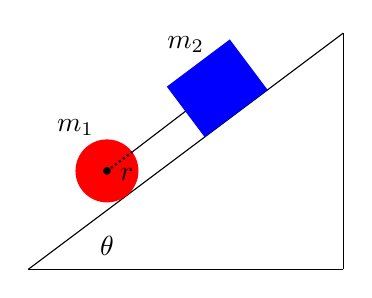
\begin{tikzpicture}
			\draw (0,0) -- (4,0);
			\draw (0,0) -- (4,3);
			\draw (4,0) -- (4,3);
			\draw (1,0.3) node {$\theta$};
			\fill[red] (1,1.25) circle (0.4);
			\fill[black] (1,1.25) circle (0.05);
			\draw (0.6,1.8) node {$m_1$};
			\draw (1.25,1.2) node {$r$};
			\draw[thick,densely dotted] (1,1.25) -- (1.32,1.49);
			\draw (1.32,1.49) -- (2,2.01);
			\fill[blue] (2.24,1.68) -- (1.76,2.32) -- (2.56,2.92) -- (3.04,2.28) -- (2.24,1.68);
			\draw (2,2.85) node {$m_2$};
		\end{tikzpicture}
		\caption{Sketch for Problem 1}
		\label{sketch_2_1_1}
	\end{figure}\\ \\
	\textbf{Solution}\\
	\begin{figure}[!hbtp]
		\centering
		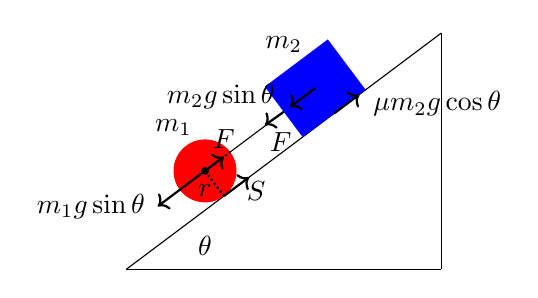
\begin{tikzpicture}
			\draw (0,0) -- (4,0);
			\draw (0,0) -- (4,3);
			\draw (4,0) -- (4,3);
			\draw (1,0.3) node {$\theta$};
			\fill[red] (1,1.25) circle (0.4);
			\fill[black] (1,1.25) circle (0.05);
			\draw (0.6,1.8) node {$m_1$};
			\draw[thick,densely dotted] (1,1.25) -- (1.24,0.93);
			\draw (1,1) node {$r$};
			\draw[thick,->] (1.24,0.93) -- (1.56,1.17);
			\draw (1.65,1) node {$S$};
			\draw[thick,densely dotted] (1,1.25) -- (1.32,1.49);
			\draw[thick,->] (1,1.25) -- (0.4,0.8);
			\draw (-0.45,0.8) node {$m_1g\sin\theta$};
			\draw[thick,->] (1,1.25) -- (1.24,1.43);
			\draw (1.24,1.65) node {$F$};
			\draw[thick,->] (2,2) -- (1.76,1.83);
			\draw (1.96,1.62) node {$F$};
			\draw (1.32,1.49) -- (2,2);
			\fill[blue] (2.24,1.68) -- (1.76,2.32) -- (2.56,2.92) -- (3.04,2.28) -- (2.24,1.68);
			\draw (2,2.85) node {$m_2$};
			\draw[thick,->] (2.4,2.3) -- (2.08,2.06);
			\draw (1.2,2.2) node {$m_2g\sin\theta$};
			\draw[thick,->] (2.64,1.98) -- (2.96,2.22);
			\draw (3.95,2.1) node {$\mu m_2g\cos\theta$};
		\end{tikzpicture}
		\caption{Auxiliary sketch for Problem 1}
		\label{sketch_2_1_2}
	\end{figure}\\ \\
	If the cord is stressed, the cylinder and the block are moving with the same acceleration $a$. Let $F$ be the tension in the cord, $S$ the frictional force between the cylinder and the inclined plane (Figure \ref{sketch_2_1_2}). The angular acceleration of the cylinder is $\alpha=\frac{a}{r}$. The net force causing the acceleration of the block
	\begin{equation*}
		m_2a=m_2g\sin\theta-\mu m_2g\cos\theta+F
	\end{equation*}
	and the net force causing the acceleration of the cylinder
	\begin{equation*}
		m_1a=m_1g\sin\theta-S-F
	\end{equation*}
	The equation of motion for the rotation of the cylinder
	\begin{equation*}
		Sr=\alpha I=\frac{a}{r}I
	\end{equation*}
	where $I$ is the moment of inertia of the cylinder, $Sr$ is the torque of the frictional force.\par
	Solving the system of equations we get
	\begin{IEEEeqnarray}{c}
		a=g\frac{(m_1+m_2)\sin\theta-\mu m_2\cos\theta}{m_1+m_2+\frac{I}{r^2}}\label{2.1.acceleration} \\
		S=\frac{I}{r^2}g\frac{(m_1+m_2)\sin\theta-\mu m_2\cos\theta}{m_1+m_2+\frac{I}{r^2}}\label{2.1.friction}\\
		F=m_2g\frac{\mu\Big(m_1+\frac{I}{r^2}\Big)\cos\theta-\frac{I\sin\theta}{r^2}}{m_1+m_2+\frac{I}{r^2}}\label{2.1.force}
	\end{IEEEeqnarray}\par
	The moment of inertia of a solid cylinder is $I=\frac{m_1r^2}{2}$. Using the given numerical values,
	\begin{IEEEeqnarray*}{c}
		a=3.25\text{ms}^{-2}\\
		S=13.01\text{N}\\
		F=0.192\text{N}
	\end{IEEEeqnarray*}\\
	\emph{Discussion}\par
	The condition for the system to start moving is $a>0$. Inserting $a=0$ into Equation (\ref{2.1.acceleration}), we obtain the limit for angle $\theta_1$
	\begin{IEEEeqnarray*}{c}
		\tan \theta_1=\mu\frac{m_2}{m_1+m_2}=\frac{\mu}{3}=0.0667\\
		\theta_1\approx3.81^{\circ}
	\end{IEEEeqnarray*}
	For the cylinder separately $\theta_1=0$ and for the block separately $\theta_1=\tan^{-1}\mu=11.31^{\circ}$. See Figure \ref{sketch_2_1_3}!
	\begin{figure}[!hbtp]
		\centering
		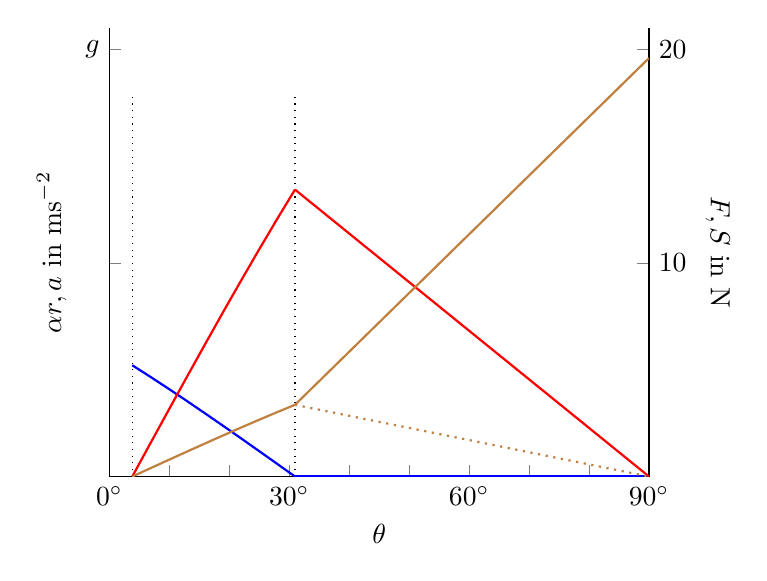
\begin{tikzpicture}
			\begin{axis}[xmin=0,xmax=90,xtick={0,10,...,90},xticklabels={0$^{\circ}$,,,30$^{\circ}$,,,60$^{\circ}$,,,90$^{\circ}$},axis x line*=bottom,ymin=0,ymax=21,ytick={0,10,20},yticklabels={,,$g$},axis y line*=left,xlabel=$\theta$,ylabel={$\alpha r,a \text{ in ms}^{-2}$},ylabel near ticks]
			\end{axis}
			\begin{axis}[xmin=0,xmax=90,hide x axis,ymin=0,ymax=21,axis y line*=right,ytick={0,10,20},yticklabels={,10,20},ylabel={$F,S\text{ in N}$},ylabel near ticks,ylabel style={rotate=180}]
				\addplot [dotted] coordinates {(3.81,0) (3.81,18)};
				\draw (38.1,190) node {$\theta_1$};
				\addplot [dotted] coordinates {(30.96,0) (30.96,18)};
				\draw (309.6,190) node {$\theta_2=\theta_3$};
				\addplot [domain=3.81:30.96,samples=10,blue,thick] {5.88*cos(x)-9.8*sin(x)};
				\draw [blue] (190,37) node {$F$};
				\addplot [blue,thick] coordinates {(30.96,0) (90,0)};
				\addplot [domain=3.81:30.96,samples=10,red,thick] {29.4*sin(x)-1.96*cos(x)};
				\draw [red] (190,95) node {$S$};
				\addplot [red,thick] coordinates {(30.96,13.44) (90,0)};
				\addplot [domain=3.81:30.96,samples=10,brown,thick] {7.35*sin(x)-0.49*cos(x)};
				\draw [brown] (270,38) node {$a$};
				\addplot [brown,thick,dotted] coordinates {(30.96,3.36) (90,0)};
				\draw [brown] (580,29) node {$\alpha r$};
				\addplot [brown,thick] coordinates {(30.96,3.36) (90,19.6)};
			\end{axis}
		\end{tikzpicture}
		\caption{Auxiliary sketch for the discussion section of Problem 1}
		\label{sketch_2_1_3}
	\end{figure}
	If the cord is not stretched the bodies move separately. We obtain the limit by inserting $F=0$ into Equation (\ref{2.1.force}),
	\begin{IEEEeqnarray*}{c}
		\tan \theta_2=\mu\Big(1+\frac{m_1r^2}{I}\Big)=3\mu=0.6\\
		\theta_2\approx30.96^{\circ}
	\end{IEEEeqnarray*}\par
	The condition for the cylinder to slip is that the value of $S$ (calculated from Equation (\ref{2.1.force}) taking the same coef\mbox{}f\mbox{}icient of friction) exceeds the value of $\mu m_1g\cos\theta$. This gives the same value for $\theta_3$ as we had for $\theta_2$. The acceleration of the centers of the cylinder and the block is the same $g(\sin\theta-\mu\cos\theta)$, the frictional force at the bottom of the cylinder is $\mu m_1g\cos\theta$, the peripheral acceleration of the cylinder is $\mu \frac{m_1r^2}{I}g\cos\theta$.
	\subsection*{Problem 2}
	There are 300$\text{cm}^3$ toluene of 0$^{\circ}\mathrm{C}$ temperature in a glass and 110$\text{cm}^3$ toluene of 100$^{\circ}\mathrm{C}$ temperature in another glass. Find the f\mbox{}inal volume after the two liquids are mixed. The coef\mbox{}f\mbox{}icient of volume expansion of toluene $\beta=0.001(^{\circ}\mathrm{C})^{-1}$. Neglect the loss of heat.\\ \\
	\textbf{Solution}\\
	If the volume at temperature $t_1$ is $V_1$, then the volume at temperature 0$^{\circ}\mathrm{C}$ is
	\begin{equation*}
		V_{10}=\frac{V_1}{1+\beta t_1}
	\end{equation*}
	In the same way, if the volume at temperature $t_2$ is $V_2$, we have
	\begin{equation*}
		V_{20}=\frac{V_2}{1+\beta t_2}
	\end{equation*}
	Furthermore, if the density of the liquid at 0$^{\circ}\mathrm{C}$ is $\rho$, then the masses are
	\begin{equation*}
		m_1=V_{10}\rho\text{ and }m_2=V_{20}\rho
	\end{equation*}
	respectively.\par
	After mixing the liquids, the temperature is
	\begin{equation*}
		t=\frac{m_1 t_1+m_2 t_2}{m_1 + m_2}
	\end{equation*}\par
	The volumes at this temperature are
	\begin{equation*}
		V_{10}(1+\beta t)\text{ and }V_{20}(1+\beta t)
	\end{equation*}\par
	The sum of the volumes after mixing
	\begin{IEEEeqnarray*}{rcl}
		V_{10}(1+\beta t)+V_{20}(1+\beta t)&\text{ }=\text{ }&V_{10}+V_{20}+\beta(V_{10}+V_{20})t\\
		&=&V_{10}+V_{20}+\beta\Big(\frac{m_1+m_2}{d}\Big)\Big(\frac{m_1t_1+m_2t_2}{m_1+m_2}\Big)\\
		&=&V_{10}+V_{20}+\beta\Big(\frac{m_1t_1+m_2t_2}{d}\Big)\\
		&=&V_{10}+\beta V_{10}t_1+V_{20}+\beta V_{20}t_2\\
		&=&V_{10}(1+\beta t_1)+V_{20}(1+\beta t_2)\\
		&=&V_1+V_2
	\end{IEEEeqnarray*}\par
	The sum of the volumes is constant. In our case, it is 410cm$^3$. The result is valid for any number of quantities of toluene, as the mixing can be done successively adding always one more glass of liquid to the mixture.
	\subsection*{Problem 3}
	Parallel light rays are falling on the plane surface of a semi-cylinder made of glass, at an angle of 45$^{\circ}$, in such a plane which is perpendicular to the axis of the semi-cylinder (Figure \ref{sketch_2_3_1}). Index of refraction is $\sqrt{2}$. Where are the rays emerging out of the cylindrical surface?
	\begin{figure}[!hbtp]
		\centering
		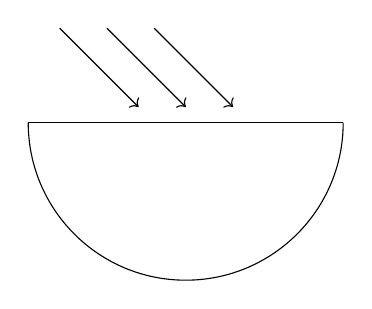
\begin{tikzpicture}
			\draw (0,0) arc (180:360:2);
			\draw (0,0) -- (4,0);
			\draw [->] (1.6,1.2) -- (2.6,0.2);
			\draw [->] (1,1.2) -- (2,0.2);
			\draw [->] (0.4,1.2) -- (1.4,0.2);
		\end{tikzpicture}
		\caption{Sketch for Problem 3}
		\label{sketch_2_3_1}
	\end{figure}\\ \\
	\textbf{Solution}\\
	Let us use angle $\theta$ to describe the position of the rays in the glass (Figure \ref{sketch_2_3_2}). According to the law of refraction, $\frac{\sin 45^{\circ}}{\sin \beta}=\sqrt{2}$, $\sin\beta=0.5$, $\beta=30^{\circ}$. The refracted angle is $30^{\circ}$ for all of the incoming rays. We have to investigate what happens if $\theta$ changes from $0^{\circ}$ to $180^{\circ}$.\par
	\begin{figure}[!hbtp]
		\centering
		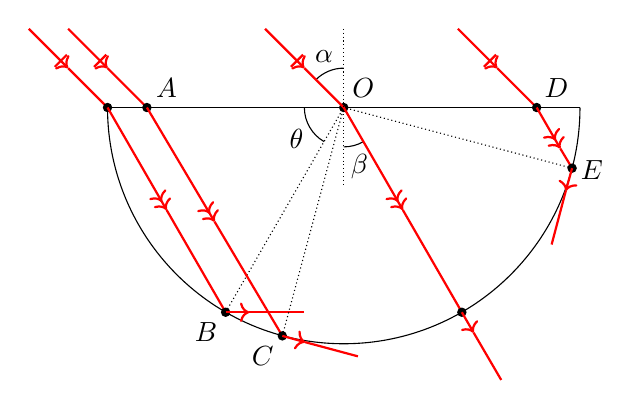
\begin{tikzpicture}
			\draw (0,0) arc (180:360:3);
			\draw (3,0.5) arc (90:135:0.5);
			\draw (2.75,0.65) node {$\alpha$};
			\draw (2.5,0) arc (180:240:0.5);
			\draw (2.4,-0.4) node {$\theta$};
			\draw (3,-0.5) arc (270:300:0.5);
			\draw (3.2,-0.75) node {$\beta$};
			\fill (3,0) circle (0.06);
			\draw (3.25,0.25) node {$O$};
			\draw (0,0) -- (6,0);
			\draw [red,thick,-|>] (-1,1) -- (-0.5,0.5);
			\draw [red,thick] (-0.5,0.5) -- (0,0);
			\fill (0,0) circle (0.06);
			\draw [red,thick,->>] (0,0) -- (0.75,-1.3);
			\draw [red,thick] (0.75,-1.3) -- (1.5,-2.6);
			\fill (1.5,-2.6) circle (0.06);
			\draw (1.25,-2.85) node {$B$};
			\draw [densely dotted] (1.5,-2.6) -- (3,0);
			\draw [red,thick,->] (1.5,-2.6) -- (1.8,-2.6);
			\draw [red,thick] (1.8,-2.6) -- (2.5,-2.6);
			\draw [red,thick,-|>] (-0.5,1) -- (0,0.5);
			\draw [red,thick] (0,0.5) -- (0.5,0);
			\fill (0.5,0) circle (0.06);
			\draw (0.75,0.25) node {$A$};
			\draw [red,thick,->>] (0.5,0) -- (1.36,-1.45);
			\draw [red,thick] (1.36,-1.45) -- (2.22,-2.9);
			\fill (2.22,-2.9) circle (0.06);
			\draw (1.97,-3.15) node {$C$};
			\draw [densely dotted] (2.22,-2.9) -- (3,0);
			\draw [red,thick,->] (2.22,-2.9) -- (2.51,-2.98);
			\draw [red,thick] (2.51,-2.98) -- (3.18,-3.16);
			\draw [red,thick,-|>] (2,1) -- (2.5,0.5);
			\draw [red,thick] (2.5,0.5) -- (3,0);
			\draw [red,thick,->>] (3,0) -- (3.75,-1.3);
			\draw [red,thick] (3.75,-1.3) -- (4.5,-2.6);
			\fill (4.5,-2.6) circle (0.06);
			\draw [red,thick,->] (4.5,-2.6) -- (4.65,-2.86);
			\draw [red,thick] (4.65,-2.86) -- (5,-3.46);
			\draw [densely dotted] (3,1) -- (3,-1);
			\draw [red,thick,-|>] (4.45,1) -- (4.95,0.5);
			\draw [red,thick] (4.95,0.5) -- (5.45,0);
			\fill (5.45,0) circle (0.06);
			\draw (5.7,0.25) node {$D$};
			\draw [red,thick,->>] (5.45,0) -- (5.75,-0.52);
			\draw [red,thick] (5.75,-0.52) -- (5.9,-0.77);
			\fill (5.9,-0.77) circle (0.06);
			\draw (6.15,-0.8) node {$E$};
			\draw [densely dotted] (5.9,-0.77) -- (3,0);
			\draw [red,thick,->] (5.9,-0.77) -- (5.82,-1.06);
			\draw [red,thick] (5.82,-1.06) -- (5.64,-1.74);
		\end{tikzpicture}
		\caption{Auxiliary Sketch for Problem 3}
		\label{sketch_2_3_2}
	\end{figure}
	It is easy to see that $\theta$ ($\angle AOB$) can not be less than $60^{\circ}$. The critical angle is given by $\sin \beta_{critical}=\frac{1}{n}=\frac{\sqrt{2}}{2}$, hence $\beta_{critical}=45^{\circ}$. In the case of total internal ref\mbox{}lection, $\angle ACO=45^{\circ}$, hence $\theta=180^{\circ}-60^{\circ}-40^{\circ}=75^{\circ}$. If $\theta$ is more than 75$^{\circ}$, the rays can emerge the cylinder. Increasing the angle we reach the critical angle again if $\angle OED=45^{\circ}$. Thus, the rays are leaving the glass cylinder if $75^{\circ}<\theta<165^{\circ}$. CE, arc of the emerging rays, subtends a central angle of 90$^{\circ}$.
\section*{Experimental problem}
	Three closed boxes (black boxes) with two plug sockets on each are present for investigation. The participants have to f\mbox{}ind out, without opening the boxes, what kind of elements are in them and measure their characteristic properties. AC and DC meters (their internal resistance and accuracy are given) and AC 50Hz and DC sources are put at the participants' disposal.\\ \\
	\textbf{Solution}\\
	No voltage is observed at any of the plug sockets therefore none of the boxes contains a source.\par
	Measuring the resistances using f\mbox{}irst AC then DC, one of the boxes gives the same result. Conclusion: the box contains a simple resistor. Its resistance is determined by measurement.\par
	One of the boxes has a very great resistance for DC but conducts AC well. It contains a capacitor, the value can be computed as $C=\frac{1}{\omega X_C}$.\par
	The third box conducts both AC and DC, its resistance for AC is greater. It contains a resistor and an inductor connected in series. The values of the resistance and the inductance can be computed from the measurements.
\chapter*{III IPhO (Brno, 1969)}
\addcontentsline{toc}
{chapter}{III IPhO (Brno, 1969)}
\section*{Theoretical problem}
	\subsection*{Problem 1}
	Figure \ref{sketch_3_1_1} shows a mechanical system consisting of three carts $A$, $B$ and $C$ of masses $m_1=0.3\text{kg}$, $m_2=0.2\text{kg}$, $m_3=1.5\text{kg}$, respectively. Carts $B$ and $A$ are connected by a light taut inelastic string which passes over a light smooth pulley attaches to the cart $C$ as shown. For this problem, all resistive and frictional forces may be ignored as may the moments of inertia of the pulley and of the wheels of all three carts. Take the acceleration due to gravity $g$ to be 9.81ms$^{-2}$.
	\begin{figure}
		[!hbtp]
		\centering
		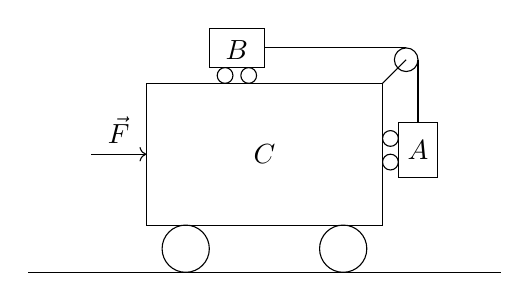
\begin{tikzpicture}
			\draw (0,0) -- (6,0);
			\draw (2,0.3) circle (0.3);
			\draw (4,0.3) circle (0.3);
			\draw (1.5,0.6) -- (4.5,0.6);
			\draw (4.5,0.6) -- (4.5,2.4);
			\draw (4.5,2.4) -- (1.5,2.4);
			\draw (1.5,2.4) -- (1.5,0.6);
			\draw (2.5,2.5) circle (0.1);
			\draw (2.8,2.5) circle (0.1);
			\draw (2.3,2.6) -- (3,2.6);
			\draw (3,2.6) -- (3,3.1);
			\draw (3,3.1) -- (2.3,3.1);
			\draw (2.3,3.1) -- (2.3,2.6);
			\draw (4.6,1.7) circle (0.1);
			\draw (4.6,1.4) circle (0.1);
			\draw (4.7,1.9) -- (4.7,1.2);
			\draw (4.7,1.2) -- (5.2,1.2);
			\draw (5.2,1.2) -- (5.2,1.9);
			\draw (5.2,1.9) -- (4.7,1.9);
			\draw (3,2.85) -- (4.8,2.85);
			\draw (4.95,1.9) -- (4.95,2.7);
			\draw (4.5,2.4) -- (4.8,2.7);
			\draw (4.8,2.7) circle (0.15);
			\draw [->] (0.8,1.5) -- (1.5,1.5);
			\draw (1.15,1.8) node {$\vec{F}$};
			\draw (3,1.5) node {$C$};
			\draw (2.65,2.82) node {$B$};
			\draw (4.95,1.55) node {$A$};
		\end{tikzpicture}
		\caption{Sketch for Problem 1}
		\label{sketch_3_1_1}
	\end{figure}\par
	A horizontal force $\vec{F}$ is now applied to cart $C$ as shown. The size of $\vec{F}$ is such that carts $A$ and $B$ remain at rest relative to cart $C$. Find the tension in the string connecting carts $A$ and $B$. Determine the magnitude of $\vec{F}$.\par
	Later, cart $C$ is held stationary, while carts $A$ and $B$ are released from rest. Determine the accelerations of carts $A$ and $B$. Calculate also the tension in the string.\\ \\
	\textbf{Solution}\\
	Case 1. The force $\vec{F}$ has so big magnitude that the carts $A$ and $B$ remain at the rest with respect to the cart $C$, i.e. they are moving with the same acceleration as the cart $C$ is. Let $\vec{G_1}$, $\vec{T_1}$ and $\vec{T_2}$ denote forces acting on particular carts as shown in the Figure \ref{sketch_3_1_2} and let us write the equations of motion for the carts $A$ and $B$ and also for whole mechanical system. Note that certain internal forces (viz. normal reactions) are not shown.
		\begin{figure}
		[!hbtp]
		\centering
		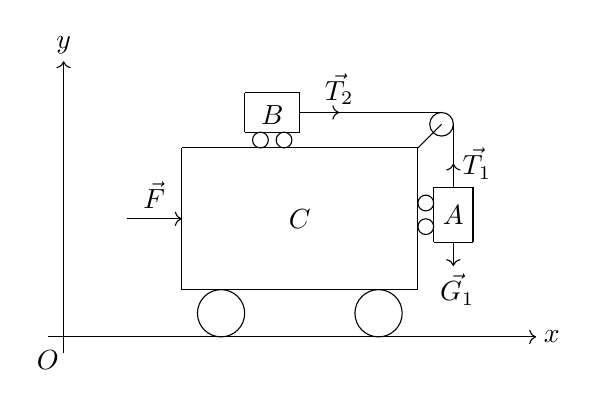
\begin{tikzpicture}
			\draw [->] (-0.2,0) -- (6,0);
			\draw [->] (0,-0.2) -- (0,3.5);
			\draw (-0.2,-0.3) node {$O$};
			\draw (0,3.7) node {$y$};
			\draw (6.2,0) node {$x$};
			\draw (2,0.3) circle (0.3);
			\draw (4,0.3) circle (0.3);
			\draw (1.5,0.6) -- (4.5,0.6);
			\draw (4.5,0.6) -- (4.5,2.4);
			\draw (4.5,2.4) -- (1.5,2.4);
			\draw (1.5,2.4) -- (1.5,0.6);
			\draw (2.5,2.5) circle (0.1);
			\draw (2.8,2.5) circle (0.1);
			\draw (2.3,2.6) -- (3,2.6);
			\draw (3,2.6) -- (3,3.1);
			\draw (3,3.1) -- (2.3,3.1);
			\draw (2.3,3.1) -- (2.3,2.6);
			\draw (4.6,1.7) circle (0.1);
			\draw (4.6,1.4) circle (0.1);
			\draw (4.7,1.9) -- (4.7,1.2);
			\draw (4.7,1.2) -- (5.2,1.2);
			\draw (5.2,1.2) -- (5.2,1.9);
			\draw (5.2,1.9) -- (4.7,1.9);
			\draw [->] (4.95,1.2) -- (4.95,0.9);
			\draw (5,0.6) node {$\vec{G_1}$};
			\draw [->] (3,2.85) -- (3.5,2.85);
			\draw (3.5,3.15) node {$\vec{T_2}$};
			\draw (3.5,2.85) -- (4.8,2.85);
			\draw [->] (4.95,1.9) -- (4.95,2.2);
			\draw (5.25,2.2) node {$\vec{T_1}$};
			\draw (4.95,2.2) -- (4.95,2.7);
			\draw (4.5,2.4) -- (4.8,2.7);
			\draw (4.8,2.7) circle (0.15);
			\draw [->] (0.8,1.5) -- (1.5,1.5);
			\draw (1.15,1.8) node {$\vec{F}$};
			\draw (3,1.5) node {$C$};
			\draw (2.65,2.82) node {$B$};
			\draw (4.95,1.55) node {$A$};
		\end{tikzpicture}
		\caption{Auxiliary Sketch for Problem 1}
		\label{sketch_3_1_2}
	\end{figure}\par
	The cart $B$ is moving in the coordinate system $Oxy$ with an acceleration $a_x$. The only force acting on the cart $B$ is the force $\vec{T_2}$, thus
	\begin{equation*}
		T_2=m_2a_x
	\end{equation*}\par
	Since $\vec{T_1}$ and $\vec{T_2}$ denote tensions in the same cord, their magnitudes satisfy
	\begin{equation*}
		T_1=T_2
	\end{equation*}\par
	The forces $\vec{T_1}$ and $\vec{G_1}$ act on the cart $A$ in the direction of the $y$-axis. Since, according to condition 1, the carts $A$ and $B$ are at rest with respect to the cart $C$, the acceleration in the direction of the $y$-axis equals to zero, $a_y=0$, which yields
	\begin{equation*}
		T_1-m_1g=0
	\end{equation*}\par
	Consequently,
	\begin{equation}
		T_1=T_2=m_1g
	\end{equation}\par
	So, the motion of the whole mechanical system is described by the equation
	\begin{equation*}
		F=(m_1+m_2+m_3)a_x
	\end{equation*}
	because forces between the carts $A$ and $C$ and also between the carts $B$ and $C$ are internal forces with respect to the system of all three bodies. Let us remark here that also the tension $\vec{T_2}$ is the internal force with respect to the system of all bodies, as can be easily seen from the analysis of forces acting on the pulley. From equations regarding tensions in the cord, we obtain
	\begin{equation*}
		a_x=\frac{m_1}{m_2}g
	\end{equation*}\par
	Substituting the last result, we arrive at
	\begin{equation}
		F=(m_1+m_2+m_3)\frac{m_1}{m_2}g
	\end{equation}\par
	Numerically,$T_2=T_1=0.3\times9.81\text{N}=2.94\text{N}$, $F=2\times\frac{3}{2}\times9.81\text{N}=29.4\text{N}$.\par
	Case 2. If the cart $C$ is immovable then the cart $A$ moves with an acceleration $a_y$ and the cart $B$ with an acceleration $a_x$. Since the cord is inextensible (i.e. it cannot lengthen), the equality
	\begin{equation*}
		a_x=-a_y=a
	\end{equation*}
	holds true. Then the equation of motion for the carts $A$, respectively $B$, can be written in the following form
	\begin{IEEEeqnarray*}{rcl}
		T_1&\text{ }=\text{ }&G_1-m_1a\\
		T_2&=&m_2a
	\end{IEEEeqnarray*}\par
	The magnitudes of the tensions in the cord again satisfy
	\begin{equation*}
		T_1=T_2
	\end{equation*}
	These yield
	\begin{equation*}
		(m_1+m_2)a=m_1g
	\end{equation*}\par
	Using the last result, we can calculate
	\begin{IEEEeqnarray}{rcl}
		a=a_x=-a_y&\text{ }=\text{ }&\frac{m_1}{m_1+m_2}g\\
		T_1=T_2&=&\frac{m_2m_1}{m_2+m_1}g
	\end{IEEEeqnarray}\par
	Numerically, $a=a_x=\frac{3}{5}\times9.81\text{ms}^{-2}=5.89\text{ms}^{-2}$, $T_1=T_2=1.18\text{N}$.
	\subsection*{Problem 2}
	Water of mass $m_2$ is contained in a copper calorimeter of mass $m_1$. Their common temperature is $t_2$. A piece of ice of mass $m_3$ and temperature $t_3<0^{\circ}\mathrm{C}$ is dropped into the calorimeter. Determine the temperature and masses of water and ice in the equilibrium state for general values of $m_1$, $m_2$, $m_3$, $t_2$ and $t_3$. Write equillibrium equations for all possible processes which have to be considered. Find the f\mbox{}inal temperature and f\mbox{}inal masses of water and ice for $m_1=1.00\text{kg}$, $m_2=1.00\text{kg}$, $m_3=2.00\text{kg}$, $t_2=10^{\circ}\mathrm{C}$, $t_3=-20^{\circ}\mathrm{C}$.\par
	Neglect the energy losses, assume the normal barometric pressure. Specif\mbox{}ic heat of copper is $c_1=0.1\frac{\text{kcal}}{\text{kg}^{\circ}\mathrm{C}}$, specif\mbox{}ic heat of water $c_2=1\frac{\text{kcal}}{\text{kg}^{\circ}\mathrm{C}}$, specif\mbox{}ic heat of ice $c_3=0.492\frac{\text{kcal}}{\text{kg}^{\circ}\mathrm{C}}$, latent heat of fusion of ice $l=78.7\frac{\text{kcal}}{\text{kg}}$. Take 1cal = 4.2J.\\ \\
	\textbf{Solution}\\
	We use the following notation: $t$ temperature of the f\mbox{}inal equillibrium state, $t_0=0^{\circ}\mathrm{C}$ the melting point of ice under normal pressure conditions, $M_2$ f\mbox{}inal mass of water, $M_3$ f\mbox{}inal mass of ice, $m^{'}_2\leq m_2$ mass of water which freezes to ice, $m^{'}_3\leq m_3$ mass of ice which melts to water.\par
	Generally, four possible processes and corresponding equilibrium states can occur:
	\begin{enumerate}
		\item $t_0<t<t_2$, $m^{'}_2=0$, $m^{'}_3=m_3$, $M_2=m_2+m_3$, $M_3=0$.\\
		Unknown f\mbox{}inal temperature $t$ can be determined from the equation
		\begin{equation}
			(m_1c_1+m_2c_2)(t_2-t)=m_3c_3(t_0-t_3)+m_3l+m_3c_2(t-t_0)
			\label{3.2.condition1}
		\end{equation}
		However, only the solution satisfying the condition $t_0<t<t_2$ does make physical sense.
		\item $t_3<t<t_0$, $m^{'}_2=m_2$, $m^{'}_3=0$, $M_2=0$, $M_3=m_2+m_3$.\\
		Unknown f\mbox{}inal temperature $t$ can be determined from the equation
		\begin{equation}
			m_1c_1(t_2-t)+m_2c_2(t_2-t_0)+m_2l+m_2c_3(t_0-t)=m_3c_3(t-t_3)
			\label{3.2.condition2}
		\end{equation}
		However, only the solution satisfying the condition $t_3<t<t_0$ does make physical sense.
		\item $t=t_0$, $m^{'}_2=0$, $0\leq m^{'}_3\leq m_3$, $M_2=m_2+m^{'}_3$, $M_3=m_3-m^{'}_3$.\\
		Unknown mass $m^{'}_3$ can be calculated from the equation
		\begin{equation}
			(m_1c_1+m_2c_2)(t_2-t_0)=m_3c_3(t-t_3)+m^{'}_3l
			\label{3.2.condition3}
		\end{equation}
		However, only the solution satisfying the condition $0<m^{'}_3<m_3$ does make physical sense.
		\item $t=t_0$, $0\leq m^{'}_2\leq m_2$, $m^{'}_3=0$, $M_2=m_2-m^{'}_2$, $M_3=m_3+m^{'}_2$.\\
		Unknown mass $m^{'}_2$ can be calculated from the equation
		\begin{equation}
			(m_1c_1+m_2c_2)(t_2-t_0)-m^{'}_2l=m_3c_3(t_0-t_3)
			\label{3.2.condition4}
		\end{equation}
		However, only the solution satisfying the condition $0<m^{'}_2<m_2$ does make physical sense.
	\end{enumerate}\par
	Substituting the particular values of $m_1$, $m_2$, $m_3$, $t_2$ and $t_3$ to Equations \ref{3.2.condition1}, \ref{3.2.condition2} and \ref{3.2.condition3}, one obtains solutions not making the physical sense (not satisfying the above conditions for $t$, respectively $m^{'}_3$). The real physical process under given conditions is given by the Equation (\ref{3.2.condition4}) which yields
	\begin{equation*}
		m^{'}_2=\frac{m_3c_3(t_0-t_3)-(m_1c_1+m_2c_2)(t_2-t_0)}{l}
	\end{equation*}\par
	Substituting given numerical values, one gets $m^{'}_2=0.11\text{kg}$. Hence, $t=0^{\circ}\mathrm{C}$, $M_2=m_2-m^{'}_2=0.89\text{kg}$, $M_3=m_3-m^{'}_2=2.11\text{kg}$.
	\subsection*{Problem 3}
	A small charged ball of mass $m$ and charge $q$ is suspended from the highest point of a ring of radius $R$ by means of an insulating cord of negligible mass. The ring is made of a rigid wire of negligible cross section and lies in a vertical plane. One the ring, there is uniformly distributed charge $Q$ of the same sign as $q$. Determine the length $l$ of the cord so as the equilibrium position of the ball lies on the symmetry axis perpendicular to the plane of the ring. Find f\mbox{}irst the general solution and then for particular values $Q=q=9.0\times10^{-8}\text{C}$, $R=5\text{cm}$, $m=1.0\text{g}$, $\epsilon_0=8.9\times10^{-12}\frac{\text{F}}{\text{m}}$.\\ \\
	\textbf{Solution}\\
	In equilibrium, the cord is stretched in the direction of resultant force of $\vec{G}=m\vec{g}$ and $\vec{F}=q\vec{E}$, where $\vec{E}$ stands for the electric f\mbox{}ield strength of the ring on the axis in distance $x$ from the plane of the ring, see Figure \ref{sketch_3_3_1}. Using the triangle similarity, one can write
	\begin{equation*}
		\frac{x}{R}=\frac{Eq}{mg}
	\end{equation*}
	\begin{figure}
		[!hbtp]
		\centering
		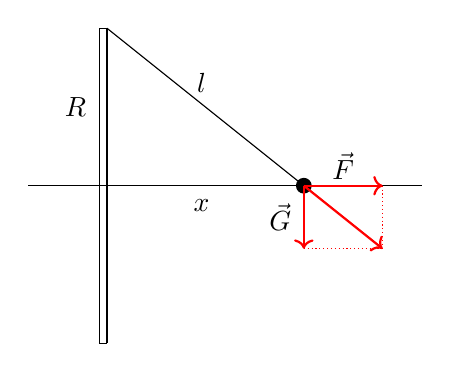
\begin{tikzpicture}
			\draw (0,0) -- (5,0);
			\draw (2.2,-0.25) node {$x$};
			\draw (0.9,-2) -- (0.9,2);
			\draw (0.9,2) -- (1,2);
			\draw (1,2) -- (1,-2);
			\draw (1,-2) -- (0.9,-2);
			\draw (0.6,1) node {$R$};
			\draw (1,2) -- (3.5,0);
			\draw (2.2,1.3) node {$l$};
			\fill (3.5,0) circle (0.1);
			\draw [red,thick,->] (3.5,0) -- (4.5,-0.8);
			\draw [red,thick,->] (3.5,0) -- (3.5,-0.8);
			\draw (3.2,-0.4) node {$\vec{G}$};
			\draw [red,densely dotted] (3.5,-0.8) -- (4.5,-0.8);
			\draw [red,thick,->] (3.5,0) -- (4.5,0);
			\draw (4,0.25) node {$\vec{F}$};
			\draw [red,densely dotted] (4.5,0) -- (4.5,-0.8);
		\end{tikzpicture}
		\caption{Sketch for Problem 3}
		\label{sketch_3_3_1}
	\end{figure}\par
	For the calculation of the electric f\mbox{}ield strength, let us divide the ring to $n$ identical parts, so as every part carries the charge $\frac{Q}{n}$. The electric f\mbox{}ield strength magnitude of one part of the ring is given by
	\begin{equation*}
		\Delta E=\frac{Q}{4\pi\epsilon_0l^2n}
	\end{equation*}\par
	This electric f\mbox{}ield strength can be decomposed into the component in the direction of the $x$-axis and $y$-axis, see Figure \ref{sketch_3_3_2}. Magnitudes of both components obey
	\begin{IEEEeqnarray*}{rcl}
		\Delta E_x&\text{ }=\text{ }&\Delta E\cos\alpha=\frac{\Delta Ex}{l}\\
		\Delta E_y&=&\Delta E\sin\alpha
	\end{IEEEeqnarray*}
	\begin{figure}
		[!hbtp]
		\centering
		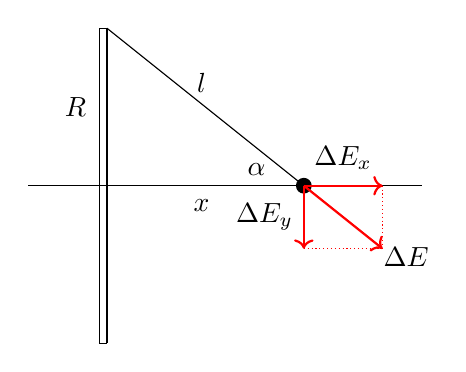
\begin{tikzpicture}
			\draw (0,0) -- (5,0);
			\draw (2.2,-0.25) node {$x$};
			\draw (0.9,-2) -- (0.9,2);
			\draw (0.9,2) -- (1,2);
			\draw (1,2) -- (1,-2);
			\draw (1,-2) -- (0.9,-2);
			\draw (0.6,1) node {$R$};
			\draw (1,2) -- (3.5,0);
			\draw (2.2,1.3) node {$l$};
			\fill (3.5,0) circle (0.1);
			\draw (2.9,0.2) node {$\alpha$};
			\draw [red,thick,->] (3.5,0) -- (4.5,-0.8);
			\draw (4.8,-0.9) node {$\Delta E$};
			\draw [red,thick,->] (3.5,0) -- (3.5,-0.8);
			\draw (3,-0.4) node {$\Delta E_y$};
			\draw [red,densely dotted] (3.5,-0.8) -- (4.5,-0.8);
			\draw [red,thick,->] (3.5,0) -- (4.5,0);
			\draw (4,0.35) node {$\Delta E_x$};
			\draw [red,densely dotted] (4.5,0) -- (4.5,-0.8);
		\end{tikzpicture}
		\caption{Auxiliary Sketch for Problem 3}
		\label{sketch_3_3_2}
	\end{figure}\par
	It follows from the symmetry, that for every part of the ring, there exists another one having the component $\Delta E_y$ of the same magnitude, but oppositely oriented. Hence, components on $y$-axis cancel each other and resultant electric f\mbox{}ield strength has the magnitude
	\begin{equation*}
		E=E_x=n\Delta E_x=\frac{Qx}{4\pi\epsilon_0l^3}
	\end{equation*}
	Finally, we obtain the cord length
	\begin{equation}
		l=\sqrt[3]{\frac{QqR}{4\pi\epsilon_0mg}}
	\end{equation}
	Numerically,
	\begin{equation*}
		l=\sqrt[3]{\frac{9.0\times10^{-8}\times9.0\times10^{-8}\times5.0\times10^{-2}}{4\pi\times8.9\times10^{-12}\times10^{-3}\times9.8}}=7.2\times10^{-2}\text{m}
	\end{equation*}
	\subsection*{Problem 4}
	A glass plate is placed above a glass cube of 2cm edges in such a way that there remains a thin air layer between them, see Figure \ref{sketch_3_4_1}. Electromagnetic radiation of wavelength between 400nm and 1150nm (for which the plate is penetrable) incident perpendicular to the plate from above is ref\mbox{}lected from both air surfaces and interferes. In this range, only two wavelengths give maximum reinforcements, one of them is $\lambda=400\text{nm}$. Find the second wavelength. Determine how it is necessary to warm up the cube so as it would touch the plate. The coef\mbox{}f\mbox{}icient of linear thermal expansion is $\alpha=8.0\times10^{-6\circ}\mathrm{C}^{-1}$, the refractive index of the air $n=1$. The distance of the bottom of the cube from the plate does not change during warming up.
	\begin{figure}
		[!hbtp]
		\centering
		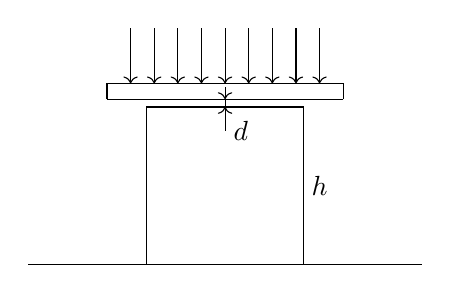
\begin{tikzpicture}
			\draw (0,0) -- (5,0);
			\draw (1.5,0) -- (1.5,2);
			\draw (3.5,0) -- (3.5,2);
			\draw (3.7,1) node {$h$};
			\draw (1.5,2) -- (3.5,2);
			\draw (1,2.1) -- (4,2.1);
			\draw (4,2.1) -- (4,2.3);
			\draw (4,2.3) -- (1,2.3);
			\draw (1,2.3) -- (1,2.1);
			\draw [->] (2.5,2.25) -- (2.5,2.1);
			\draw (2.5,2.1) -- (2.5,2);
			\draw [<-] (2.5,2) -- (2.5,1.7);
			\draw (2.7,1.7) node {$d$};
			\draw [->] (1.3,3) -- (1.3,2.3);
			\draw [->] (1.6,3) -- (1.6,2.3);
			\draw [->] (1.9,3) -- (1.9,2.3);
			\draw [->] (2.2,3) -- (2.2,2.3);
			\draw [->] (2.5,3) -- (2.5,2.3);
			\draw [->] (2.8,3) -- (2.8,2.3);
			\draw [->] (3.1,3) -- (3.1,2.3);
			\draw [->] (3.4,3) -- (3.4,2.3);
			\draw [->] (3.7,3) -- (3.7,2.3);
		\end{tikzpicture}
		\caption{Sketch for Problem 4}
		\label{sketch_3_4_1}
	\end{figure}\\ \\
	\textbf{Solution}\\
	Condition for the maximum reinforcement can be written as
	\begin{equation*}
		2dn-\frac{\lambda_k}{2}=k\lambda_k\text{ for }k=0,1,2,\dots
	\end{equation*}
	i.e.
	\begin{equation}
		2dn=(2k+1)\frac{\lambda_k}{2}
		\label{3.4.condition1}
	\end{equation}
	with $d$ being thickness of the layer, $n$ the refractive index and $k$ maximum order. Let us denote $\lambda^{'}=1150\text{nm}$. Since for $\lambda=400\text{nm}$, the condition for maximum is satisf\mbox{}ied by the assumption, let us denote $\lambda_p=400\text{nm}$, where $p$ is an unknown integer identifying the maximum order, for which
	\begin{equation}
		\lambda_p(2p+1)=4dn
		\label{3.4.condition2}
	\end{equation}
	holds true. The Equation (\ref{3.4.condition1}) yields that for f\mbox{}ixed $d$, the wavelength $\lambda_k$ increases with decreasing maximum order $k$ and vice versa. According to the assumption
	\begin{equation*}
		\lambda_{p-1}<\lambda^{'}<\lambda_{p-2}
	\end{equation*}
	i.e.
	\begin{equation*}
		\frac{4dn}{2(p-1)+1}<\lambda^{'}<\frac{4dn}{2(p-2)+1}
	\end{equation*}
	Substituting to the last inequalities for $4dn$ using Equation (\ref{3.4.condition2}), one gets
	\begin{equation*}
		\frac{\lambda_p(2p+1)}{2(p-1)+1}<\lambda^{'}<\frac{\lambda_p(2p+1)}{2(p-2)+1}
	\end{equation*}\par
	Let us f\mbox{}irst investigate the f\mbox{}irst inequality, straightforward calculations give us gradually
	\begin{equation*}
		\lambda_p(2p+1)<\lambda^{'}(2p-1)\text{ and }2p(\lambda^{'}-\lambda_p)>\lambda^{'}+\lambda_p
	\end{equation*}
	i.e.
	\begin{equation}
		p>\Bigg\lfloor\frac{1}{2}\frac{\lambda^{'}+\lambda_p}{\lambda^{'}-\lambda_p}\Bigg\rfloor=\Bigg\lfloor\frac{1}{2}\frac{1150+400}{1150-400}\Bigg\rfloor=1
		\label{3.4.condition3}
	\end{equation}\par
	Similarly, from the second inequality, we have
	\begin{equation*}
		\lambda_p(2p+1)>\lambda^{'}(2p-3)\text{ and }2p(\lambda^{'}-\lambda_p)<3\lambda^{'}+\lambda_p
	\end{equation*}
	i.e.
	\begin{equation}
		p<\Bigg\lceil\frac{1}{2}\frac{3\lambda^{'}+\lambda_p}{\lambda^{'}-\lambda_p}\Bigg\rceil=\Bigg\lceil\frac{1}{2}\frac{3\times1150+400}{1150-400}\Bigg\rceil=3
		\label{3.4.condition4}
	\end{equation}
	The only integer $p$ satisfying both Equations (\ref{3.4.condition3}) and (\ref{3.4.condition4}) is $p=2$.\par
	Let us now f\mbox{}ind the thickness $d$ of the air layer:
	\begin{equation*}
		d=\frac{\lambda_p}{4}(2p+1)=\frac{400}{4}(2\times2+1)=500\text{nm}
	\end{equation*}\par
	Substituting $d$ to the Equation \ref{3.4.condition1}, we can calculate $\lambda_{p-1}$, i.e. $\lambda_1$
	\begin{equation*}
		\lambda_1=\frac{4dn}{2(p-1)+1}=\frac{4dn}{2p-1}
	\end{equation*}\par
	Introducing the particular values, we obtain
	\begin{equation*}
		\lambda_1=\frac{4\times500\times1}{2\times2-1}=666.7\text{nm}
	\end{equation*}\par
	Finally, let us determine temperature growth $\Delta t$. Generally, $\Delta l=\alpha l\Delta t$ holds true. Denoting the cube edge by $h$, we arrive at $d=\alpha h\Delta t$. Hence
	\begin{equation*}
		\Delta t=\frac{d}{\alpha h}=\frac{5\times10^{-7}}{8\times10^{-6}\times5\times2\times10^{-2}}=3.1^{\circ}\mathrm{C}
	\end{equation*}
\chapter*{IV IPhO (Moscow, 1970)}
\addcontentsline{toc}
{chapter}{IV IPhO (Moscow, 1970)}
\section*{Theoretical problem}
	\subsection*{Problem 1}
	A long bar with mass $M=1\text{kg}$ is placed on a smooth horizontal surface of a table where it can move frictionless. A carriage equipped with a motor can slide along the upper horizontal panel of the bar, the mass of the carriage is $m=0.1\text{kg}$.
\chapter*{V IPhO (Sof\mbox{}ia, 1971)}
\addcontentsline{toc}
{chapter}{V IPhO (Sof\mbox{}ia, 1971)}
\chapter*{VI IPhO (Bucharest, 1972)}
\addcontentsline{toc}
{chapter}{VI IPhO (Bucharest, 1972)}
\chapter*{VII IPhO (Warsaw, 1974)}
\addcontentsline{toc}
{chapter}{VII IPhO (Warsaw, 1974)}
\chapter*{VIII IPhO (G\"ustrow, 1975)}
\addcontentsline{toc}
{chapter}{VIII IPhO (G\"ustrow, 1975)}
\chapter*{IX IPhO (Budapest, 1976)}
\addcontentsline{toc}
{chapter}{IX IPhO (Budapest, 1976)}
\chapter*{X IPhO (Hadrec Kr\'alov\'e, 1977)}
\addcontentsline{toc}
{chapter}{X IPhO (Hadrec Kr\'alov\'e, 1977)}
\chapter*{XI IPhO (Moscow, 1979)}
\addcontentsline{toc}
{chapter}{XI IPhO (Moscow, 1979)}
\chapter*{XII IPhO (Varna, 1981)}
\addcontentsline{toc}
{chapter}{XII IPhO (Varna, 1981)}
\chapter*{XIII IPhO (Malente, 1982)}
\addcontentsline{toc}
{chapter}{XIII IPhO (Malente, 1982)}
\chapter*{XIV IPhO (Bucharest, 1983)}
\addcontentsline{toc}
{chapter}{XIV IPhO (Bucharest, 1983)}
\chapter*{XV IPhO (Sigtuna, 1984)}
\addcontentsline{toc}
{chapter}{XV IPhO (Sigtuna, 1984)}
\chapter*{XVI IPhO (Portoro\v{z}, 1985)}
\addcontentsline{toc}
{chapter}{XVI IPhO (Portoro\v{z}, 1985)}
\chapter*{XVII IPhO (London-Harrow, 1986)}
\addcontentsline{toc}
{chapter}{XVII IPhO (London-Horrow, 1986)}
\chapter*{XVIII IPhO (Jena, 1987)}
\addcontentsline{toc}
{chapter}{XVIII IPhO (Jena, 1987)}
\chapter*{XIX IPhO (Bad Ischl, 1988)}
\addcontentsline{toc}
{chapter}{XIX IPhO (Bad Ischl, 1988)}
\chapter*{XX IPhO (Warsaw, 1989)}
\addcontentsline{toc}
{chapter}{XX IPhO (Warsaw, 1989)}
\chapter*{XXI IPhO (Groningen, 1990)}
\addcontentsline{toc}
{chapter}{XXI IPhO (Groningen, 1990)}
\chapter*{XXII IPhO (Havana, 1991)}
\addcontentsline{toc}
{chapter}{XXII IPhO (Havana, 1991)}
\chapter*{XXIII IPhO (Helsinki-Espoo, 1992)}
\addcontentsline{toc}
{chapter}{XXIII IPhO (Helsinki-Espoo, 1992)}
\chapter*{XXIV IPhO (Williamsburg, 1993)}
\addcontentsline{toc}
{chapter}{XXIV IPhO (Williamsburg, 1993)}
\chapter*{XXV IPhO (Beijing, 1994)}
\addcontentsline{toc}
{chapter}{XXV IPhO (Beijing, 1994)}
\chapter*{XXVI IPhO (Canberra, 1995)}
\addcontentsline{toc}
{chapter}{XXVI IPhO (Canberra, 1995)}

\end{document}